\documentclass[3p,authoryear,preprint,review,12pt]{elsarticle} 
\usepackage{lipsum}
\makeatletter
\def\ps@pprintTitle{%
 \let\@oddhead\@empty
 \let\@evenhead\@empty
 \def\@oddfoot{}%
 \let\@evenfoot\@oddfoot}
\makeatother
\usepackage{natbib,amssymb,amsmath,latexsym,makeidx,lscape,epic,overpic,graphicx,graphics,bm,pdflscape,rotating,multirow,bigdelim,color,epsfig,pgfpages} \usepackage{mathpazo}
\usepackage{mathtools}
\usepackage[portuguese, english]{babel}
\usepackage[T1]{fontenc}
\usepackage[utf8]{inputenc}
\usepackage[left]{eurosym}
\usepackage{pdfsync,epstopdf,dblfloatfix,multicol,wrapfig,multirow}
\usepackage{epstopdf}
\usepackage{units}
\epstopdfsetup{outdir=./}
\usepackage[draft]{hyperref} % Drop [draft] to have references hyperlinked.
\usepackage{float}
\usepackage{longtable,booktabs}
\usepackage[toc,page]{appendix}
\usepackage{url}

\newcommand{\squeezeup}{\vspace{-2pt}}
\setlength{\textfloatsep}{3pt plus 1.0pt minus 2.0pt}
       \setlength{\abovecaptionskip }{-1ex} 

%Standard settings for an Elsevier article. 
\def\elsartstyle{\def\normalsize{\@setfontsize\normalsize\@xiipt{12.5}} \def\small{\@setfontsize\small\@xipt{13.6}} \let\footnotesize=\small
   \def\large{\@setfontsize\large\@xivpt{18}} \def\Large{\@setfontsize\Large\@xviipt{22}}  \skip\@mpfootins = 18\p@ \@plus 2\p@ \normalsize }
    
       
\begin{document}

\begin{frontmatter}
 \title{Public transport and school location impacts on educational inequalities: insights from São Paulo}
   
  \author[uab]{Ana~I.~Moreno-Monroy}
 \ead{anaisabel.moreno@uab.cat}
 
  \author[uol]{Robin Lovelace}
  
   \author[fgv]{Frederico R. Ramos}
  
 \address[urv]{Applied Economics Department, Autonomous University of Barcelona}
  \address[uol]{Intitute of Trasnport Studies, University of Leeds}
 \address[fgv]{CEPESP, Fundação Getulio Vargas}

\begin{abstract}
In many large Latin American urban areas such as the São Paulo
Metropolitan Region (SPMR), growing social and economic inequalities are embedded through high spatial inequality in the provision of state schools and affordable public transport to these schools. This paper sheds light on the transport-education inequality nexus with reference to school accessibility by public transport in the SPMR. 
To assess school accessibility, we develop an accessibility index which combines information on the spatial distribution of adolescents, the location of existing schools, and the public transport provision serving the school catchment area into a single measure. The index is used to measure school accessibility locally across 633 areas within the SPMR. We use the index to simulate the impact of a policy aiming at increasing the centralization of public secondary education provision, and find that it negatively affects public transport accessibility for students with the lowest levels of accessibility. These results illustrate how existing inequalities can be amplified by variable accessibility to schools across income groups and geographical space.
The research suggests that educational inequality impacts of school agglomeration policies should be considered before centralisation takes place and highlights the links between transport planning social injustice that.
\end{abstract}


\begin{keyword}
Public transport, accessibility, schools, inequality, Latin America\\
\end{keyword}

\end{frontmatter}

\newpage
\section{Introduction}\label{introduction}

Inequalities in educational and transport infrastructure are mutually reinforcing: the right to mobility is intrinsically linked to the right to education. Travel to school options are vital for ensuring a more equitable supply of educational opportunity to diverse groups.Conversely, poor accessibility to and from deprived areas can reinforce social inequalities, with long-term implications. Against this background, in this paper we propose a new way to measure school accessibility in local areas within an urban area, and apply it for the case of the São Paulo Metropolitan Region (SPMR).

The SPMR presents an excellent opportunity to measure the extent of
educational and public transport provision, and to study the impact of
public policies on different socio-economic groups. Partly as a response to the pressures from the Free Pass Movement that started in March, 2013, low income public school students residing in the SPMR gained access to a public transport subsidy in 2015. However, in October 2015, the São Paulo state government announced during a television interview that as part of a budgetary deficit reduction plan, dozens of secondary schools would be closed in 2016. The change in policy was estimated to affect more than 300,000 students, many whom would be placed in schools far from their homes. As a response, in the following months students occupied over 200 schools. Protesters scored some victories: the reform was postponed for one year, and the education secretary resigned (Ortellado 2015).

Although this time the policy change was not carried out, in a context of high spatial inequalities in the provision of public transport and schooling, it is worth asking whether a public transport subsidy for students can compensate for the lower provision of public schools in some areas. In this dynamic and highly political context, new quantitative evidence can help shed light on the relationship between transport and educational inequalities and the extent to which they are mutually reinforcing. Moreover, the results should help design school location and public transport policies that are more inclusive and equitable by highlighting areas where
school location and public transport opportunities conspire to exacerbate educational inequalities.

The recent experience of São Paulo and other cities informed the paper's public transport emphasis. 
This could be seen as a contrast to the topic of active travel to school, which has gained recent prominence in Australia (e.g. Veitch et al., 2017) the USA (Lee et al., 2017) and Europe (e.g. Macdonald et al., 2016).
However, we see great potential synergies between provision of public and active transport opportunities and, by focussing on public transport, do not wish to endorse an `either or' approach to adequate school travel opportunities.
The focus on public transport is especially appropriate in a Latin American context where parents' perception of road danger may (rightly) be greater and where parents cannot be expected automatically to be able to have the resources to buy and maintain a bike for children to cycle to school (public provision of safe walking and cycling infrastructure and bicycles are areas of research worthy of attention beyond the scope of this paper).

Our proposed competitive accessibility measure combines information
about the place of residence of students, the spatial distribution of public schools, and public transport accessibility into a single
measure. We start from a cumulative opportunity measure that counts the number of schools seats that can be reached within a 30 minute journey by public transport, and then build a competitive measure that takes into account the place of residency of teens. Travel-to-school times by public transport are based on actual commuting times obtained through use of routing algorithms provided on-line through an on-line service. 

For this work we used the Google Matrix Distance API
(application programming interface), a multi-modal
real-time travel data provider (see \href{https://developers.google.com/maps/documentation/distance-matrix/}{developers.google.com/maps/}). 
The API was used in preference to other options,
such as Routino --- see Singleton (2014) for a used case involving large-scale accessibility analysis ---
and the OpenStreetMap Routing Machine (OSRM)
because its
ease of use (requiring no new software to be installed locally)
and performance: the Google Distance Matrix
API returns
route distance, price (but not price for travel to school) and times for journeys between origins and
destinations, provided either as Longitude/Latitude pairs or
as text strings to be 'geocoded' (converted to geographical location).

We calculate these measures for 633 areas within the SPMR. We use the competitive measure to simulate the impact of a policy change in the location of public secondary schools, in order to, first, understand the extent of spatial inequalities in school accessibility by public transport, and second, estimate the
effect of a policy aiming at concentrating public secondary education provision on school accessibility. We find that closing down schools in areas with lower than average provision is highly regressive: it
negatively impacts students with the lowest accessibility levels,
accentuating existing inequalities.

The first well-known quantitative definition of accessibility was by Ingram (1971).
This seminal paper presented a range of measures determined by
distances to destinations (Euclidean and network), natural barriers and 
distance decay functions. This early work made the distinction
between accessibility indices that apply to zones or single `desire
lines': ``relative accessibility is defined as a measure of the effort of overcoming spatial separation between two points, while the integral accessibility is defined as a measure of the effort of overcoming spatial separation between a point and all other points within an area'' (Allen, Liu, and Singer 1993). In subsequent works, the measurement of job accessibility by particular transport modes has received vast attention in the literature (Geurs and Van Wee 2004), while studies on access to education has largely focused on the consequences of mode choice on socio-economic indicators and school outcomes (see for instance Asahi (2014), Falch, Lujala, and Str{ø}m (2013) and Dickerson and McIntosh (2012) on the impact of accessibility on school outcomes, and Andersson, Malmberg, and {Ö}sth (2012) and Easton and Ferrari (2015) on the effect of changes in travel-to-school patterns in developed economies).

Our index is inspired by the index developed by Shen (1998) in the
context of job accessibility. The main innovative element with respect to previous proposed measures of school accessibility is that it takes into account both the `supply' and `demand' for schooling in each area. Concretely, it is based on the idea that in each local area, there is a certain amount of students in (secondary) school age, and a certain quantity of (public) school seats available. As areas are part of a city, each local area is also subject to the inflow of potential students from other areas, as well of the outflow of students to other areas. The magnitude of the net flow will depend on the travel distance between all other areas and the area in question, which here we consider to be the public transport commuting time between areas. The index thus
captures the fact that students compete for school seats, which are
limited in number, and distributed unequally across space. The inclusion of this competitive element to school accessibility, akin to that in job access, highlights the fact that under certain educational systems, the access to opportunities is mediated by competition.

Our work contributes to the literature on transport-related social
exclusion (Jones and Lucas 2012) (Lucas et al. 2016) by providing a
quantitative way to assess multiple dimensions into a single measure. Education and public transport are both essential public services, and thus are part of the set of fundamental and universal human rights. Lack of sufficient access to these services limits the way in which individuals use can their capacities and exercise their rights in a context of equal opportunities (Gomide 2003). Our index provides a benchmark to compare access inequalities in countries with unequal provision of public services (Gomide 2006), (Pacione 1989). Considering contestation as the process through which social groups mobilize in an organized way in order to impede the implementation of unwanted policies, or force the negotiation of new conditions, our index allows embedded inequalities to be better understood.

After this introduction, we detail our data sources and definitions in Section 2. Section 3 describes the area of study and presents some preliminary findings. Section 4 describes the proposed methods for measuring school accessibility. Section 5 presents the results for the SPMR, and finally, Section 6 concludes.

\section{Data}\label{data}

The school accessibility index was created using data from the following sources: 
\begin{itemize}
\item Demographic Census – 2010 – IBGE
\item Origen – Destination Survey – 2007 – Metro
\item School Census – 2008 – INEP
\item Geocoded Schools – CEM/CEBRAP – 2001
\item Geocoded Public Schools – SEADE – 2008
\item Google Distance Matrix API 
\end{itemize}

The School Census data was provided by the Brazilian National Institute of Educational Studies and Surveys (INEP).
The dataset contains information on all public educational
institutions, including a unique identifier and the number of students enrolled in secondary education. School coordinates contained in a database provided by the Center for Metropolitan Studies CEM (\textit{Centro de Estudos da Metrópole}) for 2001 were used to geolocate the schools in 2008 using the unique identifier.
To include new schools built between 2001 and 2008, we used a dataset provided by the Fundação SEADE (São Paulo State Agency for Statistical Analysis) containing the geocoded location for all state administration schools at 2008. The this dataset set was obtained merging this two data source using the standard ID used by the INEP. We geo-localized a total of 4,612 public schools in the SPMR.

The second source was the 2010 Population Census of Brazil,
compiled and freely distributed by the Brazilian Institute of Statistics (IBGE). We aggregated the data by 633 administrative zones in the SPMR: Area de Ponderacão Espacial (AEP)
areas, a spatial unit defined for surveying purposes by IBGE.
IBGE provides geographical datasets containing the boundaries of these areas. From the census microdata, we have data on the number of inhabitants by age for each enumeration area, which totals more than one million secondary school students: 1,216,611 people of secondary school age (15 - 18 years) were recorded in the Census dataset (approximately 13 percent of the population).

The final source of information was derived from the Google Distance
Matrix API, which provided travel times and distances by public
transport. This was implemented using an interface to the API by means of the R package \textbf{stplanr} (Lovelace et al. 2016). To provide an example of how the method works, a reproducible example is illustrated below.

\begin{figure}[H]
\includegraphics[width=1\linewidth]{box} \label{fig:box}
\end{figure}
\begin{verbatim}
##   distances duration
## 1      2962     2118
\end{verbatim}

The code above takes an origin (\texttt{o}) and destination (\texttt{d}) and finds the travel time and distance. This is reported as 2,962 metres and 2,118 seconds (35 minutes) respectively. To ensure that the result was relevant to school travel, the times were calculated for arrival time at 9am on a weekday. The function was repeated for all origin-destination pairs. To ensure the correct OD data was being generated, the results were plotted on an interactive map (Figure \ref{fig:pairs}).
The results show the high variability of route distance versus Euclidean distance (`circuity'), providing further evidence of inequalities in public transport provision in the city (Figure \ref{fig:euclid}).
\begin{figure}[H]
\includegraphics[width=1\linewidth]{od-map} \caption{Visual representation of the 12,697 OD pairs routed through the Google Distance Matrix API on an interactive map in RStudio, an open source data analysis platform.}\label{fig:pairs}
\end{figure}

\begin{figure}[H]
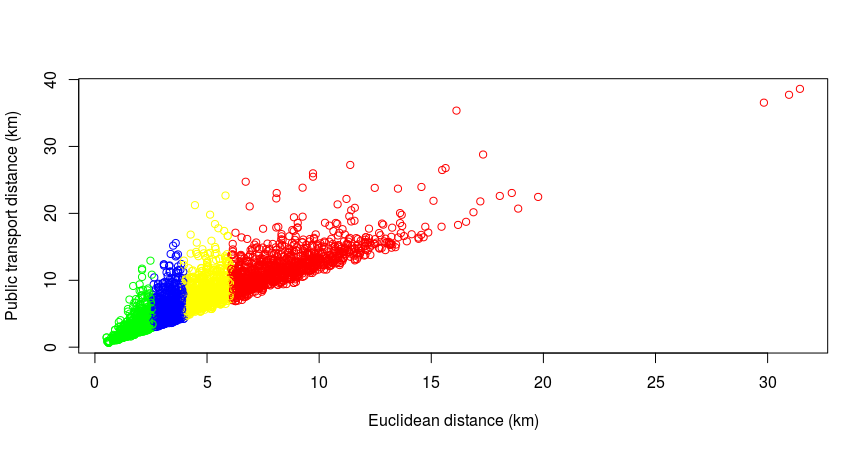
\includegraphics[width=0.5\linewidth]{public-vs-euclid-dists} \caption{Euclidean (straight line) vs public transport distances resulting from routing the 12,697 OD pairs of interest through the Google Distance Matrix API. The colours represent the interquantile range of the Euclidean distances travelled to school.}\label{fig:euclid}
\end{figure}

\section{Area of study}\label{area-of-study}

The São Paulo Metropolitan Region (SPMR) groups 38 different municipalities besides the municipality of São Paulo itself. The estimated population in 2010 was close to 19.5 million inhabitants. It has an integrated transport system, to which users can access through an electronic card (Bilhete Único) composed of a railway and bus network. The railway network comprises 78.4 kilometers in five subway lines and six suburban railway lines which provide less frequent and slower service than the subway. Some of the bus network operates on dedicated bus corridors, which amounted to 500 km in 2015. As can be seen in Figure \ref{fig:inc-trans}, the richer areas of the SPMR are better served by public transport, while an important number of lower income areas is under-served.

\begin{figure}[H]
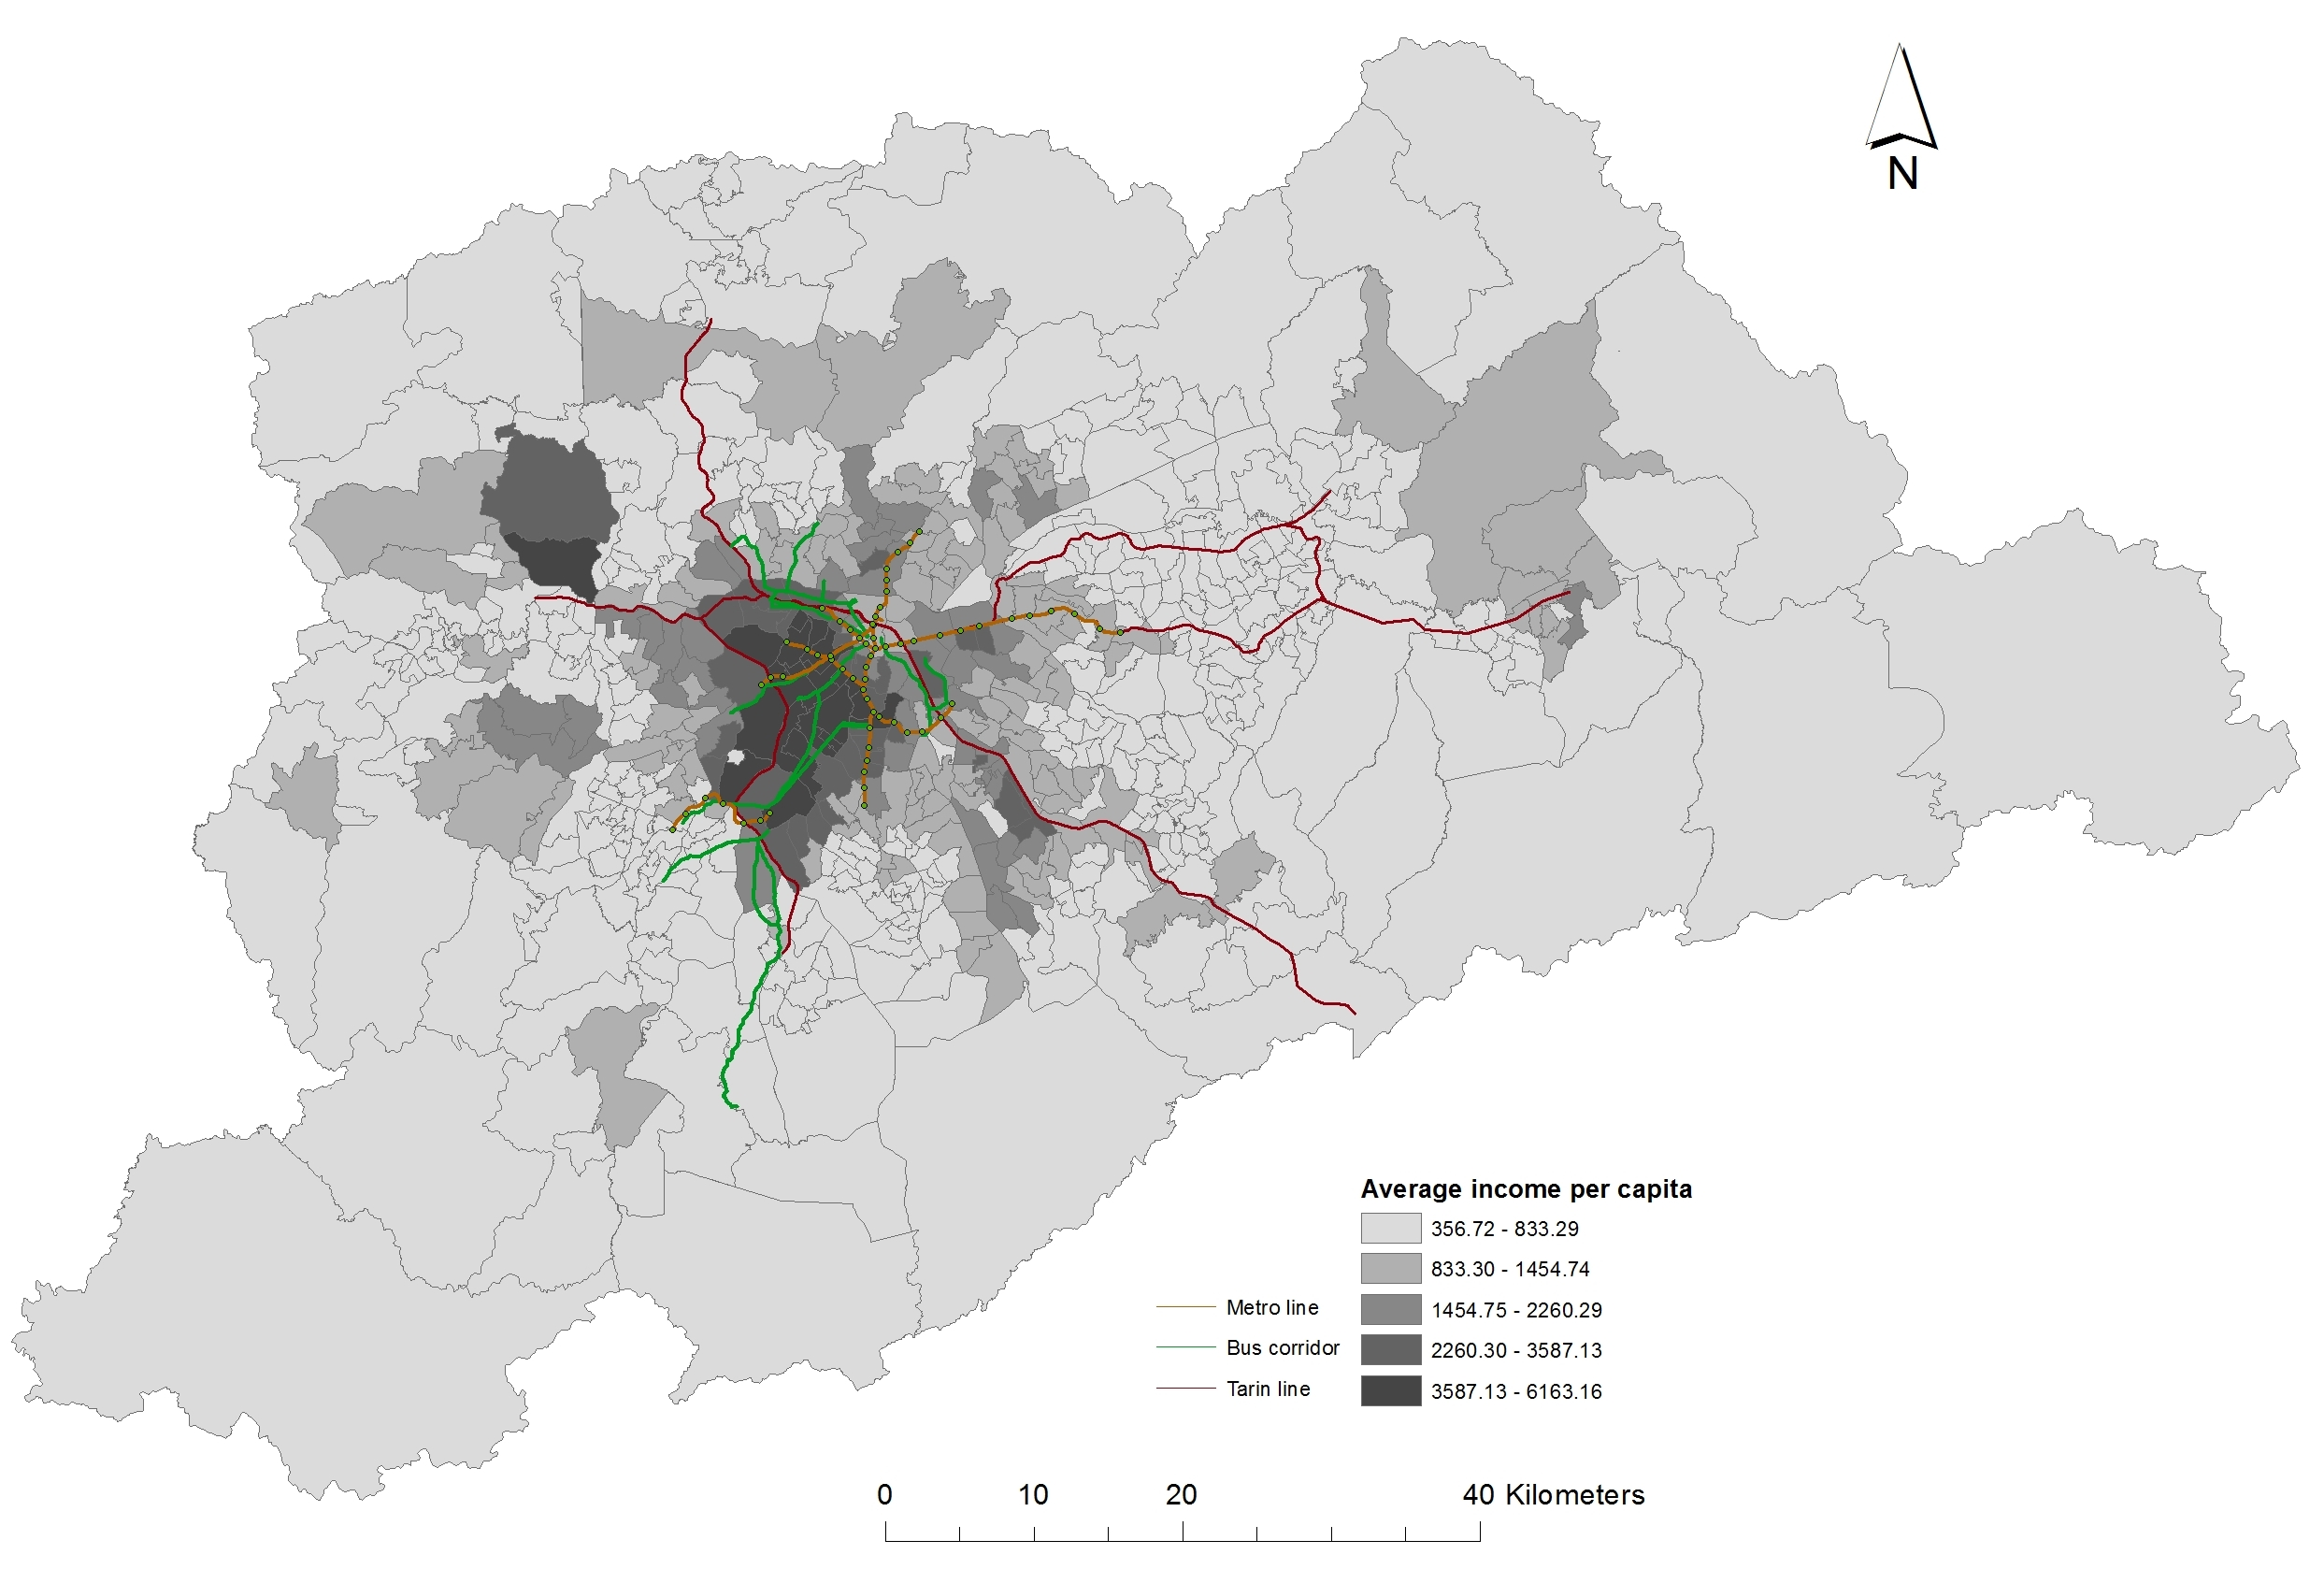
\includegraphics[width=0.8\linewidth]{income_pc} \caption{Public transport system and income per capita in São Paulo, 2010.}\label{fig:inc-trans}
\end{figure}

Regarding the educational system, primary education is compulsory. In 2005, the legislation changed to increase the duration of the primary education, going from eight to nine years. In 2010, all regions finished the transition. In 2009, a constitutional amendment imposed compulsory education for the primary and secondary levels. The constitution imposes that this resolution should be fully implemented by 2016. By law, the state/municipalities should guaranty the adequate provision (100\% coverage of the demand). There are national and state educational funds that are distributed among the schools per number of enrolled students and existence of facilities (library, laboratories, etc.). The structure of the educational system is composed by both public and private schools. The public schools are divided in the following levels: Pre school (classe de alfabetização) – 4-5 year-olds (municipal administration); Fundamental (ensino fundamental) comprises nine years, and the age range is usually 6-14 year-olds (municipal administration); Secondary (ensino médio) lasts a minimum of three years, and the age range is 15-18 year-olds (state administration); and Post-secondary (ensino superior) (state and federal administration).

According to the School Census (\textit{Censo Escolar}) 2010\footnote{see
  \url{http://portal.inep.gov.br/basica-censo} for details on the School
  Census}, there are 10,251 schools in the SPMR, out of which 54\% are public (22\% state / 32\% municipal) and 46\% are private.
Geographically, students are assigned to the closest school to their
place of residency or their parent's working place. For secondary
school, the student can ask for a vacancy in a different school after providing a valid justification and under the condition of the
availability of vacancy.

The municipality is responsible for the organization of the pre-school and fundamental level. Poorer municipalities in SPMR have, in general, lower quality in terms of teachers and facilities. All the secondary schools are administrated by the state, nevertheless, differences exists depending of the location in the SPMR. In general, schools in peripheral locations show lower quality scores.

As can be seen by comparing Figures \ref{fig:inc-trans} and \ref{fig:students}, students in the SPMR disproportionally attend private secondary schools in higher income areas, while the opposite is true for public secondary schools.

\begin{figure}[H]
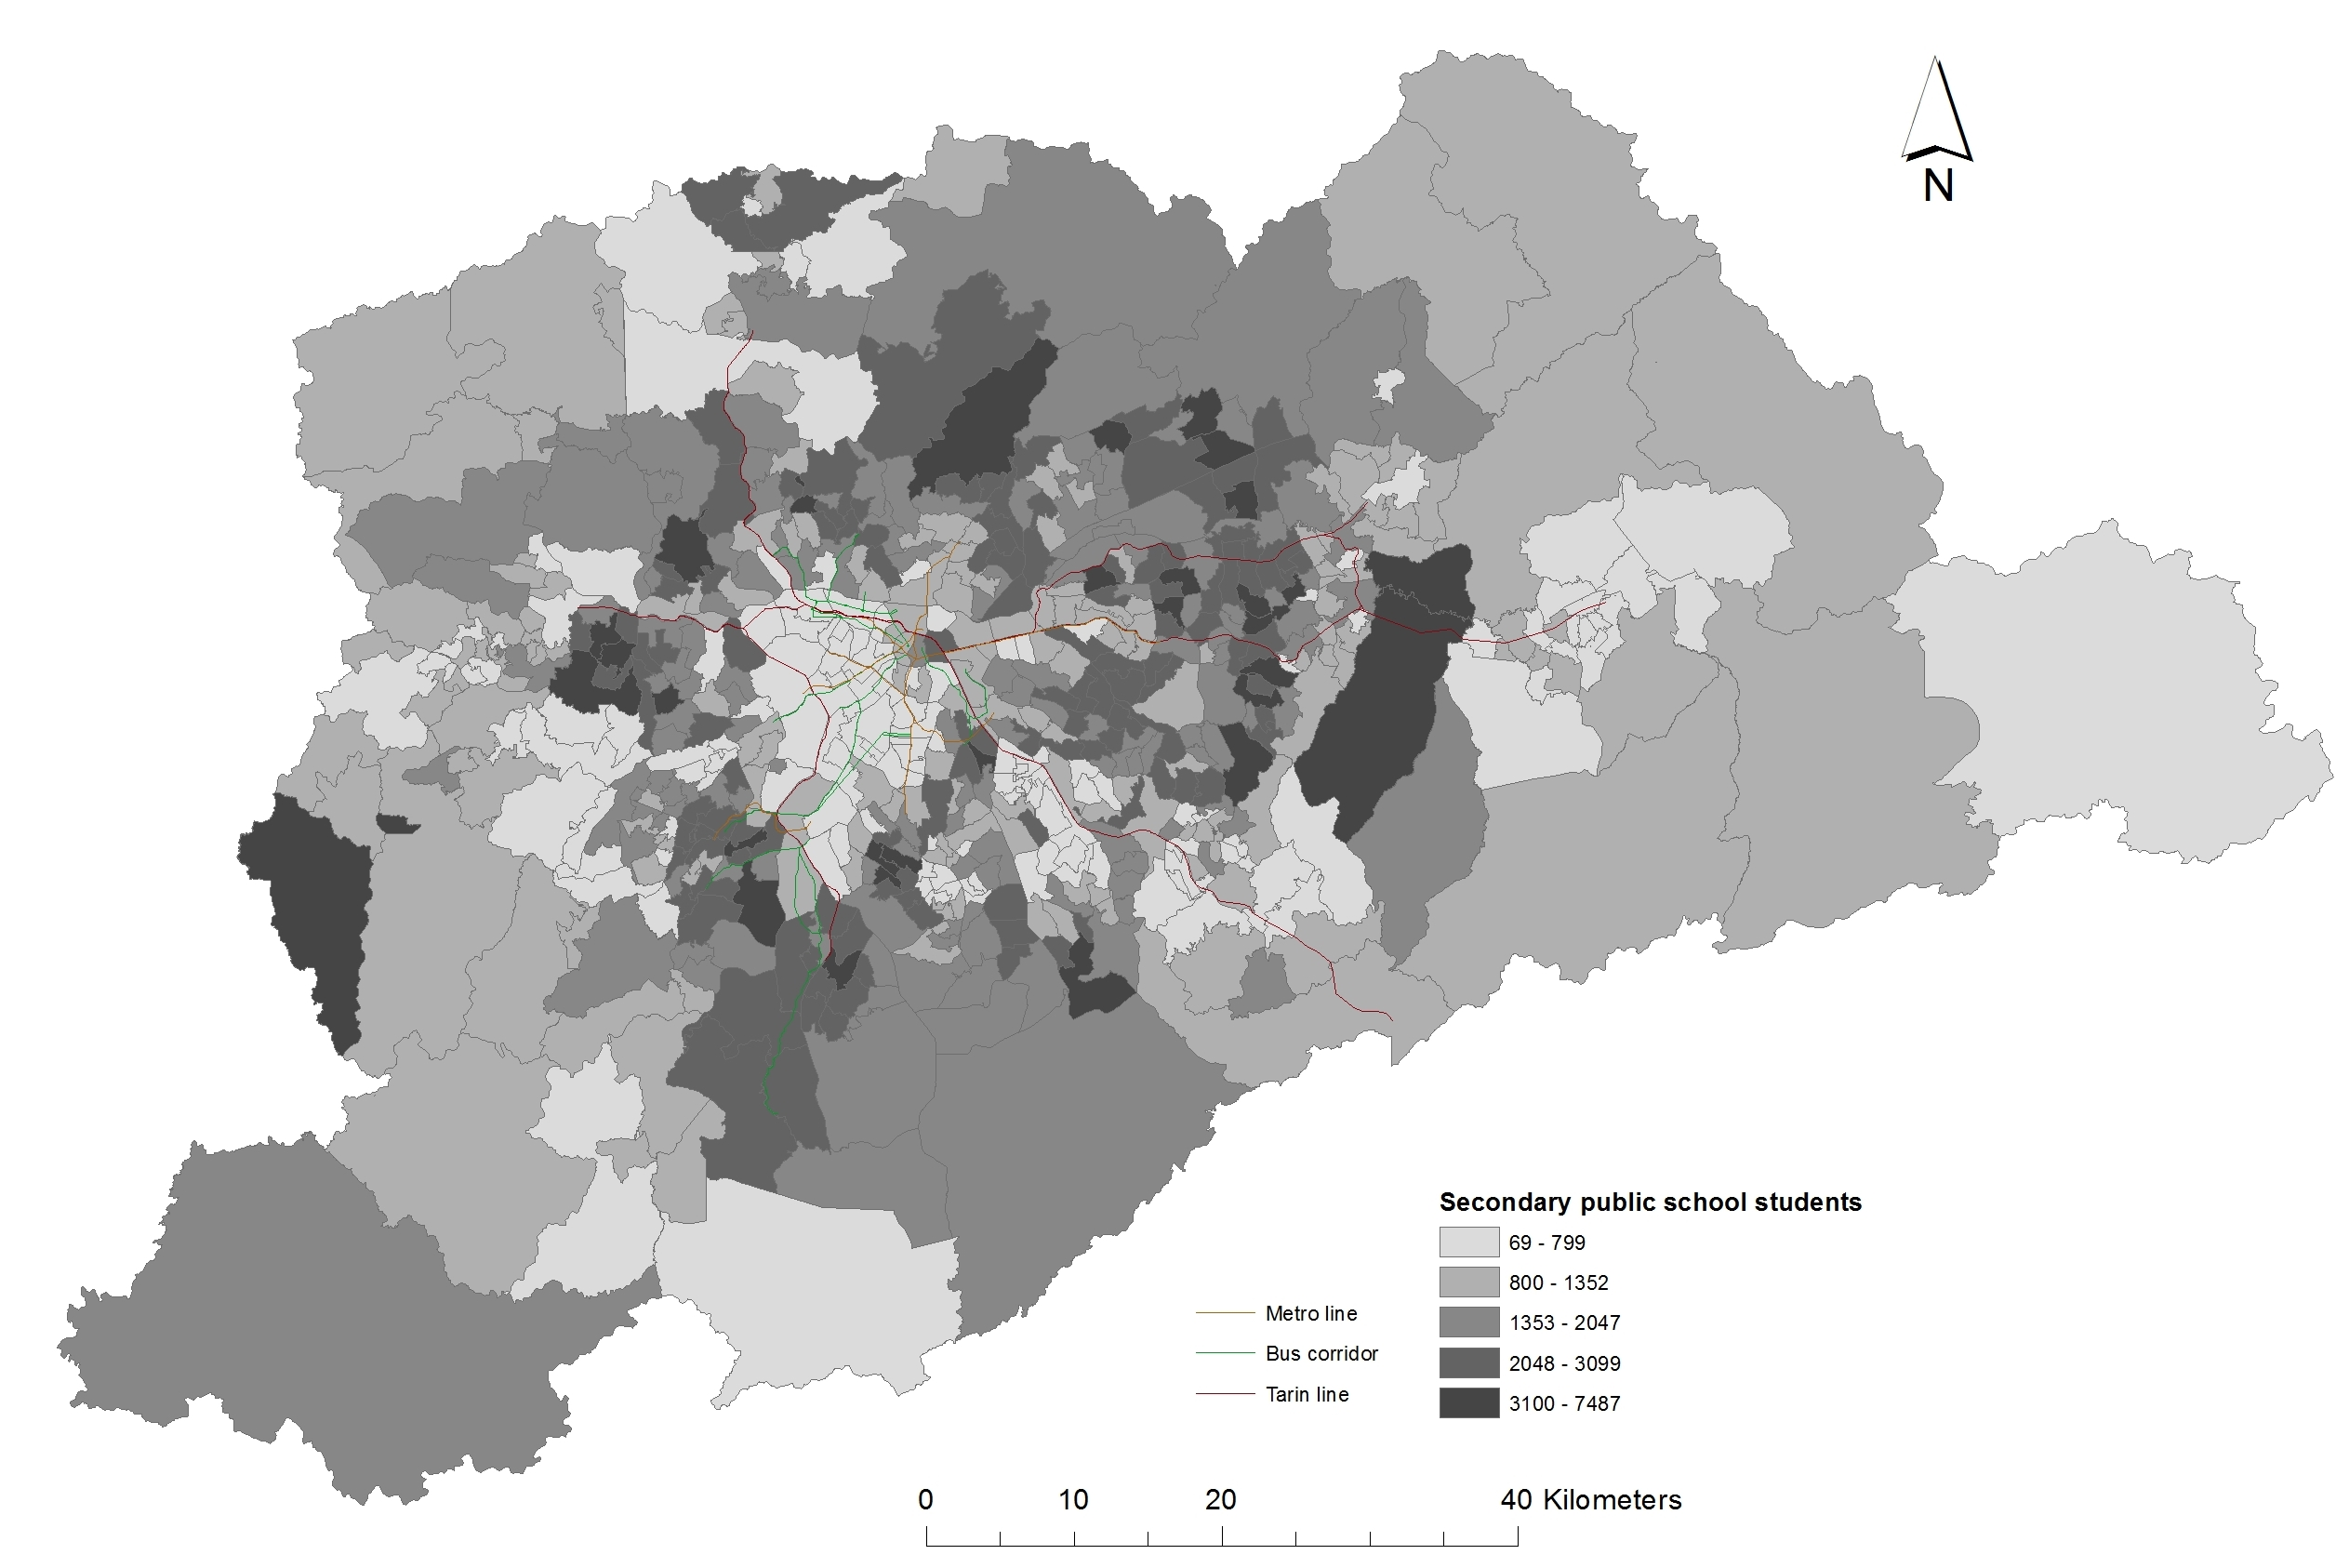
\includegraphics[width=1\linewidth]{med_pu} \caption{The home location of students attending public secondary schools students in the SPMR.}\label{fig:students}
\end{figure}

As Figure 5 shows, enrolment in public secondary schools is more
dispersed spatially, as in principle public schools are not clearly
geographically concentrated within the region. There is, however, an
important degree of variation in the school seats in each sub-area,
ranging from zero to 7,754.
\begin{figure}
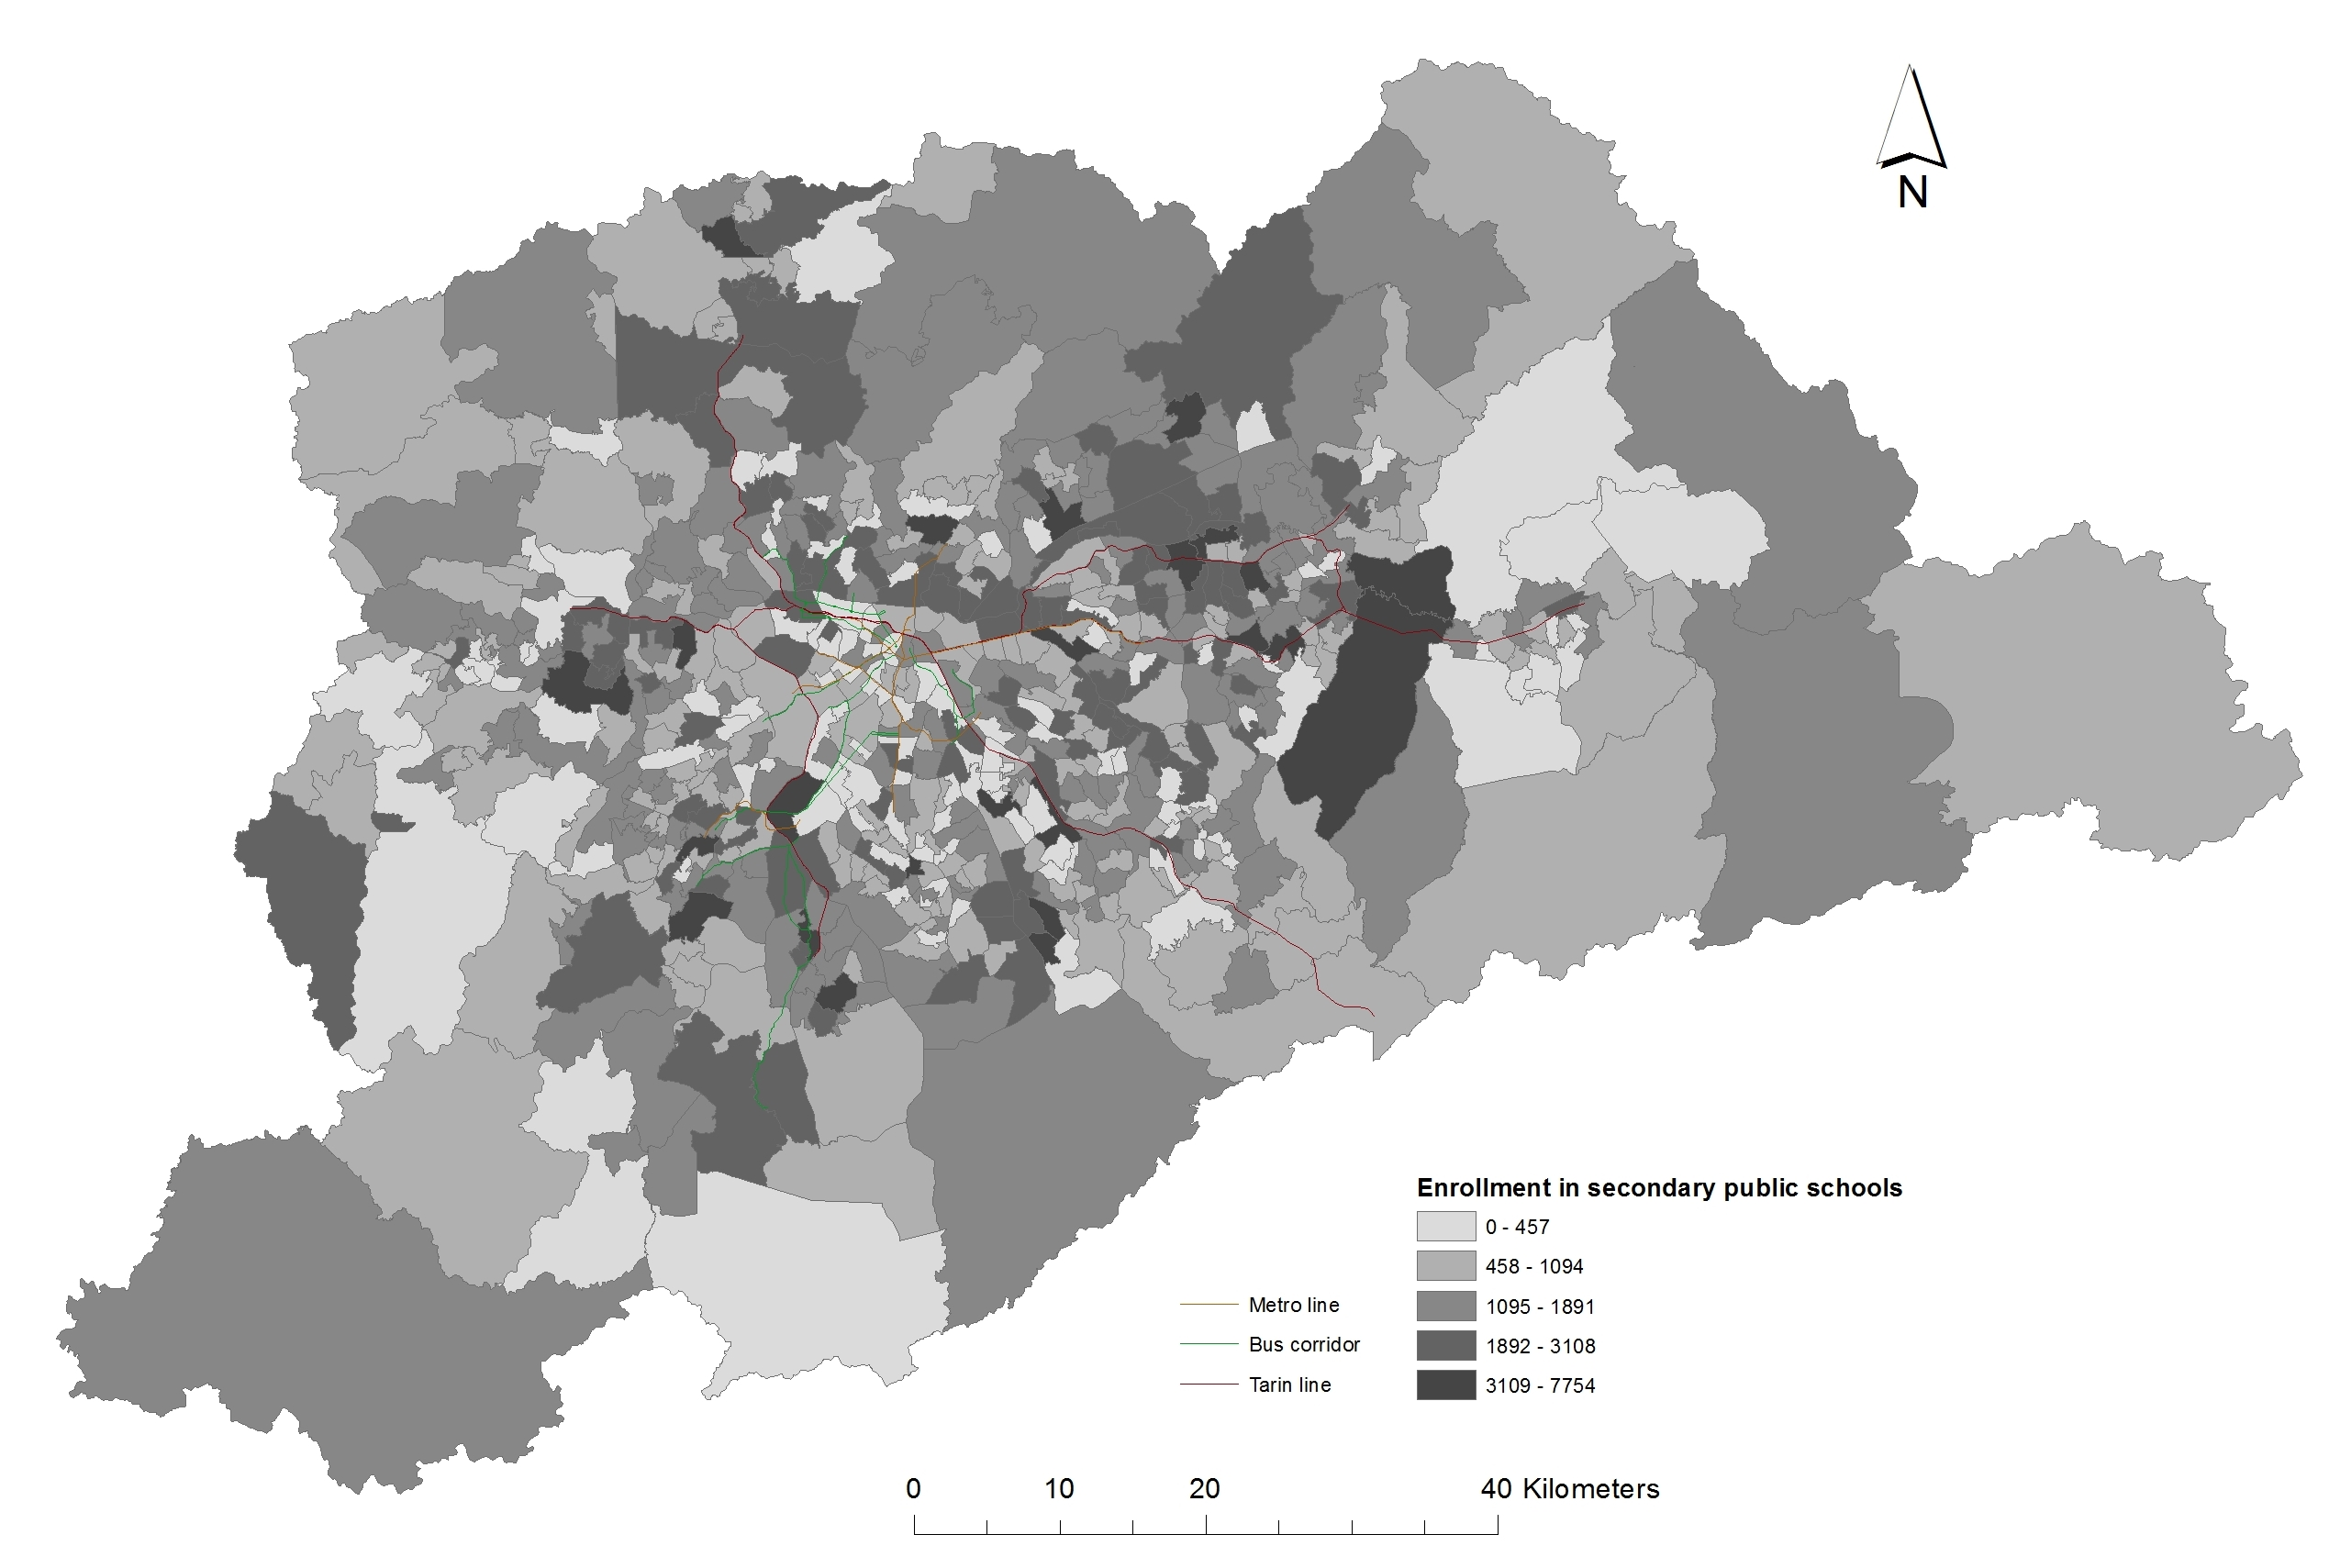
\includegraphics[width=0.7\linewidth]{enrol} \caption{Enrollment in public secondary schools in the SPMR.}\label{fig:unnamed-chunk-7}
\end{figure}
Table 1 shows the modal split by type of secondary school student.\footnote{The source of this information is the 2007 Origin-Destination Household Travel Survey (O-D Survey), carried out by the São Paulo Metropolitan Transport Authority Mêtro. We focus on   trips made by secondary school students with an indicated motive   ``education'' at the destination. The total number of trips (excluding missing values) was 11,845. Of these, 5.5 percent were multimodal. In those cases, we assign the mode of the trip leg with the largest duration. We add all trip leg durations (in minutes) to obtain the total trip duration.} 
  
Clearly, secondary school students attending private schools disproportionally travel by car, compared to public school students (47\% versus 9\%), even though higher income areas are better served by public transport. This is in line with the findings of
S{á} et al. (2015). Around 67\% of public school students commute to
school by active travel (mostly walking, since the percentage of biking is still relatively small), while 23\% commute by public transport, which has much longer mean duration than other modes. Gomide (2003), using data from the 1997 SPMR Origin-Destination survey, reports that the motive ``education'' explained at least 60\% of trips in the SPMR of individuals earning up to one minimum wage a month. This proportion decreases as income increases, as other motives such as work and leisure become more relevant.

Although the mean duration of travel to school remained stable over the period 1997-2007 (S{á} et al. 2015), travel-to-school times could increase as a result of several factors relevant to the SPMR, including sub-urbanization of particular demographic groups, such as those with higher income; increase in the size of schools leading to an increase in school's catchment area; less than proportional increase in schools in high population growth areas with poor connectivity; and institutional changes towards more flexible school choice (Easton and Ferrari 2015).

\begin{table}[H]\centering \caption{Modal split by type of secondary school}
\begin{tabular}{lcc} \hline
\multicolumn{3}{c}{\textbf{Secondary Public School Students}}  \\  \hline
 & Percent & Duration (min)  \\ \hline
Public & 23 & 36.7 \\
Private & 9 & 15.8 \\
Active & 68 & 15.7 \\ \hline
\multicolumn{3}{c}{\textbf{Secondary Private School Students}}  \\  \hline
Public & 28 & 35.7 \\ 
Private & 47 & 17.3 \\
Active & 25 & 13.9 \\\hline
\multicolumn{3}{l}{\small Public transport includes bus, metro and railway.} \\
\multicolumn{3}{l}{\small Active transport includes walking and cycling.}  
\end{tabular}
\end{table} \label{split}

\section{Method: measuring school
accessibility}\label{method-measuring-school-accessibility}

To define school accessibility, we start with the broad concept of
accessibility, as used in the transport literature. According to Geurs and Van Wee (2004) (p.~128) accessibility is ``the extent to which land-use and transport systems enable (groups of) individuals to reach activities or destinations by means of a (combination of) transport mode(s).'' Extended to our case, school accessibility then measures the extent to which the existing built-environment and transport facilities enable children and adolescents in school age to reach schools.

Ideally, a school accessibility measure would include information on the home location of every student and the location of every school they could potentially attend (as in Andersson, Malmberg, and {Ö}sth (2012)), and some measure of commuting costs for any chosen mode (in terms of time and money). Given that this level of detail is not available in our data, we rely on area aggregates, implicitly assuming that the measure at the centroid of the area applies homogeneously within the area.

Given these limitations, we first consider a cumulative-opportunity
measure for mode \(M\) (Boisjoly and El-Geneidy 2016) is defined as:

\[ CO_{i}^M= \sum_{j=1}^nO_{j}f(C_{ij}) \]

\[ f(C_{ij}) = \left\{ 
                \begin{array}{ll}
                  1\quad if\quad C_{ij}<=t\\
                  0\quad if\quad C_{ij}>t
                \end{array}
              \right.
\]

This measure counts the number of ``opportunities'' \(O\), in our case schools available, from one area within a certain travel time threshold by mode \(M\). \(C_{ij}\) is the travel cost (measured in time) between the centroid of zone \(i\) and the centroid of zone \(j\), and \(f(C_{ij})\) is a weight function.

This measure takes into account the spatial distribution of schooling opportunities, but not the local demand for schooling. This is particularly relevant for our analysis, since it could be the case that some areas are disproportionally served with respect to the number of potential students living within a certain travel distance. In order to assess the mismatch between the demand and supply for schooling, we use the sum of students in schools in each area (supply), and the sum of individuals within the school grade age-group living in each area (demand) in the following competitive accessibility measure (Shen 1998):

\[ CA_{i}^M= \sum_{j=1}^n\frac{O_{j}f(C_{ij})}{\sum_{k=1}^n(T_{k}f(C_{kj}))}\]

Where the numerator discounts the number of school seats in area \(j\), \(O_{j}\), by how far area \(i\) is from area \(j\) using the same function as before, and the denominator discounts the number of teens in secondary school age living in zone \(k\), \(T_{k}\), by how far they are from area \(j\). In other words, the numerator counts how many schools seats can be reached from an area, while the denominator counts how many teens can potentially reach the same area. In this way, the discounted number of school seats places at each area is divided by the potential students available to fill those places, and then summed in order to obtain a single accessibility measure for each area.

We calculate both measures for commutes to school by public transport. We set a threshold of 30 minutes based on the mean average travel times by this mode (see Table \ref{split}). As a robustness check, in the result sections we show results for 35 and 40 minutes thresholds. We assign a minimum time of zero for commutes within the same area (i.e., schools within the same area are added to the index in all cases).

\section{Results}\label{results}

\subsection{School accessibility}\label{results}

Figure \ref{fig:cum_ind} shows the spatial distribution of the cumulative-opportunity measure. The index has a mean value of 3,777, which indicates that for teens residing in the average area, there are 3,777 school seats that can be reached within a journey by public transport of up to 30 minutes. The standard deviation is 3,485 indicates large variation in the level of accessibility across areas.

The results show that areas with low accessibility include not
only the expanded financial business district located on the central
south west area, where higher-income teens mostly attend private school (see Figures \ref{fig:inc-trans} and \ref{fig:students}), but also areas with deficient public transport provision, such as some north and south eastern areas.

\begin{figure}[H]
\includegraphics[width=0.7\linewidth]{cum_index} \caption{Cumulative opportunity index}\label{fig:cum_ind}
\end{figure}

Figure \ref{fig:comp_ind} shows the spatial distribution of the competitive accessibility measure. Although it largely follows the distribution of the cumulative index, it corrects the value in some areas based on the place of residence of students across the SPMR. To interpret the value of the index, recall that if all teens in an area attended secondary schools in public secondary schools in their area (i.e., no student would attend private school or travel outside her own area to attend school), the index would take the value of 1. Then, in areas with a value lower than one, the provision of public schools and public transport is such that there is local under-provision, in the sense that the number of schools seats that can be reached from the area is smaller than the number of teens that can potentially reach the area (the opposite is true for values higher than one). Note that some relatively close by areas, especially in the eastern part of the city, have striking differences in the level of accessibility. In some cases, an area can have twice the level of accessibility than the most proximate area. This can be due to differences in the local provision of public schools, public transport or the number of students living within the reach of the areas.

\begin{figure}[H]
\includegraphics[width=0.7\linewidth]{comp_index} \caption{Competitive accessibility index}\label{fig:comp_ind}
\end{figure}

\subsection{Policy experiment}\label{results}

To understand the effects of changes in public school provision on
school accessibility, we conduct a comparative static analysis using our competitive index. The experiment mimics a policy that aims at increasing scale economies in the provision of public education by centralizing provision in larger educational establishments, which is the rationale behind the policy proposal made by the São Paulo state government (Ortellado 2015). In this spirit, instead of selecting a specific number of schools to be closed or students to be reallocated, we compare the changes in school-accessibility before and after the implementation of a policy that closes down schools which fall under a specified size threshold. The threshold  choice is based on the quantiles of the school size distribution of all schools in the area. Figure \ref{density} shows the density plot of the number of students and three different thresholds: 15\%, 25\% and 50\%. 

\begin{figure}[H]
\includegraphics[width=0.7\linewidth]{density} \caption{Competitive accessibility index}\label{fig:density}
\end{figure}

Table \ref{thresholds} summarizes the size threshold corresponding to each scenario, the number of schools which would close and the number of students which would be reallocated in each case. 

\begin{table}[H]\caption{Policy experiment scenarios}\label{thresholds}
\begin{tabular}[c]{lccc}\hline
Scenario & Size threshold & \# Schools closed & \# Students reallocated \\ \hline
15\% & 337 & 343 & 8,002 \\
25\% & 572 & 711 & 36,807 \\
50\% & 1,061 & 1691 & 163,231 \\\hline
\end{tabular}
\end{table}

To implement the policy experiment, we assign students in areas with
lower than average enrolment to the next area with higher than average enrolment, while keeping the distribution of teens and public transport constant. In other words, total enrolment is the same before and after the change, but the distribution of public secondary schools increases in areas where it was already higher than average, and disappears in areas where it was lower than average. In the most extreme scenario, the change is equivalent to closing down 1,691 schools, or reallocating 163,231 students. Although seemingly massive, it is worth noting again that the proposal of the São Paulo state government was estimated to impact 300,000 secondary students attending public school (Ortellado 2015). We then compare the changes in school accessibility for different quartiles before and after this change. Table \ref{policy_change} summarizes the results for a 30 minute threshold in the Competitive Accessibility Index. Table \ref{sen1} in the Appendix presents the results for 35 and 40 minutes thresholds.

\begin{longtable}[H]{@{}lrrr@{}} 
\caption{Mean accessibility before and after
redistribution}\tabularnewline
\toprule
Quantile & Pre-change & Post-change & Change (\%)\tabularnewline
\midrule
\endfirsthead
\toprule
Quantile & Pre-change & Post-change & Change (\%)\tabularnewline
\midrule
\endhead
1st & 0.446 & 0.350 & -21.566\tabularnewline
2nd & 0.844 & 0.822 & -2.592\tabularnewline
3rd & 1.843 & 2.124 & 15.213\tabularnewline
4th & 4.280 & 5.483 & 28.099\tabularnewline
\bottomrule
\end{longtable} \label{policy_change}

The policy reduces further the accessibility level of areas in the first and second quantiles of accessibility. Areas in the first quantile experience an average reduction of 21\% in school accessibility levels as a result of the changes in the spatial distribution of schools. The average reduction is 17\% and 14\% when 35 and 40 minutes thresholds are used instead of a 30 minute threshold (see Table \ref{sen1} in the Appendix). In
the mean time, areas that had high levels of accessibility to start
with, experience an increase, which varies between a maximum of 28\% for the fourth quantile when a 30 minute threshold is chosen, to 19\% when a 40 minute threshold is used instead. The results suggest that concentrating the provision of public secondary schools accentuates the already large differences in accessibility levels across areas.

\section{Conclusion and discussion}\label{conclusion-and-discussion}

The policy experiment results suggest that a policy that concentrates the provision of public schools spatially is regressive. Young people living in areas with the lowest levels of accessibility experience the largest negative impact from the policy, compounding issues of low local schooling provision, low access by public transport and/or high competition to access good schools. The policy would increase commuting times for students residing in areas with low accessibility. This would likely have further negative knock-on effects in terms of attendance,
drop-out likelihood and performance.

Although the simulated scenario represents a rather extreme change in the distribution of public schooling, the way in which students with different levels of accessibility are impacted remains, regardless of the level of concentration. In the absence of a public transport subsidy for school commutes, students who experience a substantial increase in travel-to-school times may be forced to change their commute mode from an active (and free of charge mode) to a paid-by mode, with the consequent increase in their monetary spent in commuting to school. The most negative effect is then felt by low-incomes students living in areas with low school accessibility, for whom the marginal increase in commuting costs represents a much larger share in their budget.

The provision of a public transport subsidy for school commutes is
unlikely to compensate students at the bottom of the income and
accessibility ladder if the increase in commuting times has consequences in terms of motivation to stay in school and performance. In this sense, a ``trade-off'' logic where less schooling provision is compensated by public transport subsidies does not operate when existing inequalities in provision are large.
The use of travel times rather than economic cost raises the question: is affordability or accessibility more important in affecting educational inequalities?
The focus on the time data from the Google Matrix API reflects the greater robustness of this measure (prices can fluctuate rapidly) and the fact that, thanks to the Free Pass Movement, there is a widespread perception that public transport to schools should be free. The analysis in this paper therefore assumes very low or zero financial cost for public transport to school.


Our study could be further extended to account for other modes of school commute, such as active travel. It would benefit from data with higher spatial resolution to capture within-area inequalities, which may be substantial but currently hidden away in area aggregates. A future extension of the index could also incorporate measures of school quality. Furthermore, it would be informative to calculate the proposed indices for other contexts and different time periods, to understand the extent to which the regressive nature of school agglomeration is a universal finding or specific to the SPMR.

We conclude that extending the concept of local accessibility indicators to education can help to both contest and constructively tackle embedded social inequalities. Contestation can be seen as a powerful tool to prevent the implementation of regressive policies that threaten to accentuate already large disparities. Quantitative measures such as those proposed here can help demonstrate how multiple dimensions of inequality amplify inequalities, via a single interpretable measure. The methods demonstrated could be useful for policy makers and campaigners to negotiate policies with a highly sensitive social component and evident short and long-term consequences for those affected.

\section*{Appendix}
\setcounter{figure}{0}
\renewcommand{\thefigure}{A\arabic{figure}}

\setcounter{table}{0}
\renewcommand{\thetable}{A\arabic{table}}

\begin{table}[H]\caption{Mean accessibility before and after
redistribution, different time thresholds}\label{sen1}
\begin{tabular}[c]{lcccccc}\hline
 & \multicolumn{2}{c}{Pre-change} & \multicolumn{2}{c}{Post-change} & \multicolumn{2}{c}{ Change (\%)} \\ \hline
Quantile & 35 min & 40 min & 35 min & 40 min& 35 min & 40 min \\ \hline 
1st & 0.56 & 0.638 & 0.46 & 0.55 & -16.92 & -13.61 \tabularnewline
2nd & 1.06 & 1.23 & 1.05 & 1.209 & -0.54 & -1.85 \tabularnewline
3rd & 2.22 & 2.51 & 2.52 & 2.773 & 13.64 & 10.72 \tabularnewline
4th& 5.26 & 6.69 & 7.22 & 7.928 & 37.29 & 18.55 \tabularnewline
\bottomrule
\end{tabular}
\end{table}

\begin{table}[H]\caption{Mean accessibility before and after
redistribution, different allocation rule}\label{sen2}
\begin{tabular}[c]{lccccccc}\hline
 & \multicolumn{2}{c}{Pre-change} & \multicolumn{2}{c}{Post-change} & \multicolumn{2}{c}{ Change (\%)} \\ \hline
Percentile & < 0.15  & < 0.25 &  < 0.15  & < 0.25 & < 0.15  & < 0.25 \\ \hline 
1st & 0.446 & 0.421 &  0.443 & 0.397 & -0.70 & -5.59 \tabularnewline
2nd & 0.844 & 0.832 &  0.838 & 0.820 & -0.70 & -1.42 \tabularnewline
3rd & 1.843 & 1.92 &  1.859 & 2.00 & 0.83 & 4.37 \tabularnewline
4th & 4.280 & 4.30 &  4.280 & 4.32 & 0 & 0.37 \tabularnewline
\bottomrule
\end{tabular}
\end{table}

\section{References}\label{references}

Allen, W Bruce, Dong Liu, and Scott Singer. 1993. ``Accessibility
Measures of US Metropolitan Areas.'' \emph{Transportation Research Part
B: Methodological} 27 (6). Elsevier: 439--49.

Andersson, Eva, Bo Malmberg, and John {Ö}sth. 2012. ``Travel-to-School
Distances in Sweden 2000--2006: Changing School Geography with Equality
Implications.'' \emph{Journal of Transport Geography} 23. Elsevier:
35--43.

Asahi, Kenzo. 2014. ``The Impact of Better School Accessibility on
Student Outcomes.'' The London School of Economics; Political Science,
SERC Discussion Paper.

Boisjoly, Genevi{è}ve, and Ahmed El-Geneidy. 2016. ``Daily Fluctuations
in Transit and Jobs Availability: A Comparative Assessment of
Time-Sensitive Accessibility Measures.'' \emph{Journal of Transport
Geography}, no. 52: 73--81.

Dickerson, Andy, and Steven McIntosh. 2012. ``The Impact of Distance to
Nearest Education Institution on the Post-Compulsory Education
Participation Decision.'' \emph{Urban Studies}. SAGE Publications,
0042098012455717.

Easton, Sue, and Ed Ferrari. 2015. ``Children's Travel to School---the
Interaction of Individual, Neighbourhood and School Factors.''
\emph{Transport Policy} 44. Elsevier: 9--18.

Falch, Torberg, P{ä}ivi Lujala, and Bjarne Str{ø}m. 2013. ``Geographical
Constraints and Educational Attainment.'' \emph{Regional Science and
Urban Economics} 43 (1). Elsevier: 164--76.

Geurs, Karst T, and Bert Van Wee. 2004. ``Accessibility Evaluation of
Land-Use and Transport Strategies: Review and Research Directions.''
\emph{Journal of Transport Geography} 12 (2). Elsevier: 127--40.

Gomide, Alexandre de {Á}vila. 2003. ``Transporte Urbano E Inclusão
Social: Elementos Para Políticas Públicas.'' Instituto de Pesquisa
Econômica Aplicada (Ipea).

---------. 2006. ``Mobilidade Urbana, Iniqüidade E Políticas Sociais.''
Instituto de Pesquisa Econômica Aplicada (Ipea).

Ingram, David R. 1971. ``The Concept of Accessibility: A Search for an
Operational Form.'' \emph{Regional Studies} 5 (2). Taylor \& Francis:
101--7.

Jones, Peter, and Karen Lucas. 2012. ``The Social Consequences of
Transport Decision-Making: Clarifying Concepts, Synthesising Knowledge
and Assessing Implications.'' \emph{Journal of Transport Geography} 21.
Elsevier: 4--16.

Lee, Richard J., Ipek N. Sener, and S. Nathan Jones. 2017. ``Understanding the Role of Equity in Active Transportation Planning in the United States.'' \emph{Transport Reviews} 37 (2): 211–26.

Lovelace, Robin, Richard Ellison, Barry Rowlingson, and Nick Bearman.
2016. \emph{Stplanr: Sustainable Transport Planning}.
\url{https://github.com/ropensci/stplanr}.

Lucas, Karen, John Bates, Jos{é} Moore, and Juan Antonio Carrasco. 2016.
``Modelling the Relationship Between Travel Behaviours and Social
Disadvantage.'' \emph{Transportation Research Part A: Policy and
Practice} 85. Elsevier: 157--73.

Macdonald, Laura, Paul McCrorie, Natalie Nicholls, and Anne Ellaway. 2016. ``Walkability around Primary Schools and Area Deprivation across Scotland.'' \emph{BMC Public Health} 16: 328.

Ortellado, Pablo. 2015. ``Brazil's Students Occupy Their Schools to Save
Them.'' \emph{The New York Times}, 15 December 2015. Available:
http://www.nytimes.com/2015/12/16/opinion/brazils-students-occupy-their-schools-to-save-them.html?\textsubscript{r}=1
{[}Last accessed: 25 April 2016{]},

Pacione, Michael. 1989. ``Access to Urban Services---the Case of
Secondary Schools in Glasgow.'' \emph{The Scottish Geographical
Magazine} 105 (1). Taylor \& Francis: 12--18.

S{á}, Thiago H{é}rick de, Leandro Martin Totaro Garcia, Gr{é}gore Iven
Mielke, Fabiana Maluf Rabacow, and Leandro F{ó}rnias Machado de Rezende.
2015. ``Changes in Travel to School Patterns Among Children and
Adolescents in the São Paulo Metropolitan Area, Brazil, 1997--2007.''
\emph{Journal of Transport \& Health} 2 (2). Elsevier: 143--50.

Singleton, Alex. 2014. ``A GIS approach to modelling CO2 emissions associated with the pupil-school commute.'' \emph{International Journal of Geographical Information Science} 28, 256–273. doi:10.1080/13658816.2013.832765

Shen, Qing. 1998. ``Location Characteristics of Inner-City Neighborhoods
and Employment Accessibility of Low-Wage Workers.'' \emph{Environment
and Planning B: Planning and Design} 25 (3). SAGE Publications: 345--65.

Veitch, J., A. Carver, J. Salmon, G. Abbott, K. Ball, D. Crawford, V. Cleland, and A. Timperio. 2017. ``What Predicts Children’s Active Transport and Independent Mobility in Disadvantaged Neighborhoods?'' \emph{Health \& Place} 44 (March): 103–9. doi:10.1016/j.healthplace.2017.02.003.


\end{document}
